\subsection{Teilversuch 1: Polarisatoren und Gesetz von Malus}
	
		\subsubsection*{Methoden}
			
			\begin{figure}[ht]
				\centering
				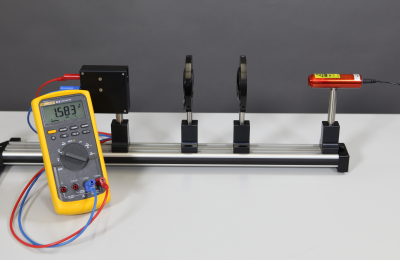
\includegraphics[width=\textwidth]{bilder/Polarisation.png}
				\caption{Aufbau des ersten Teilversuches\cite{WWU}}
				\label{fig:Polarisation}	
			\end{figure}
			Der Aufbau des ersten Teilversuches ist in Abb. \ref{fig:Polarisation} dargestellt.
			Zunächst soll jedoch nur einer der Polarisatoren zwischen dem Laser und der Photodiode stehen.
			Diese soll so gedreht werden, dass die gemessene Spannung maximal ist.
			Dann soll der zweite Polarisator hinzugefügt werden und ausgehend von dem gleichen Winkel wie bei dem ersten in \SI{10}{\degree} Schritten bis \SI{+-90}{\degree} von dem Ausgangswinkel die Spannung gemessen werden.
			Dies dient zu der Überprüfung des Gesetzes von Malus, welches sich wie folgt definiert:
			\begin{equation}
				I = I_0 \cos^2{\phi}.
			\end{equation}
			Dabei ist $I$ die gemessene Intensität, $I_0$ die Ausgangsintensität und $\phi$ der Winkel um den der zweite Polariseur gedreht sein soll.
			Da jedoch Spannung betrachtet werden sollen, werden statt $I$ und $I_0$ gerade $U$ und $U_0$ betrachtet, was aufgrund der Proportionalität von $I$ und $U$ ebenfalls dem Gesetz von Malus genügen sollte.
			
		\subsubsection*{Durchführung}
		
			Der Winkel, bei dem die gemessene Spannung bei nur einem Polarisator maximal war, belief sich auf $\phi_0 = \SI{106+-0,4}{\degree}$.
			So wurden nach dem Einfügen des zweiten Polarisators die Spannungen für die Winkel $\phi = \SIrange{16+-0,4}{196+-0,4}{\degree}$ gemessen.
			Hierbei ließ sich beobachten, dass ausgehend von $\phi_0$ bei zunehmendem und abnehmendem Winkel die Intensität kleiner wurde.
			Zudem wurden die Minima an den beiden Enden der Messungen verzeichnet.
			Abb. \ref{fig:PolarisationFit} beinhaltet die gemessenen Werte.
		
		\subsubsection*{Datenanalyse}
			
			\begin{figure}[ht]
				\centering
				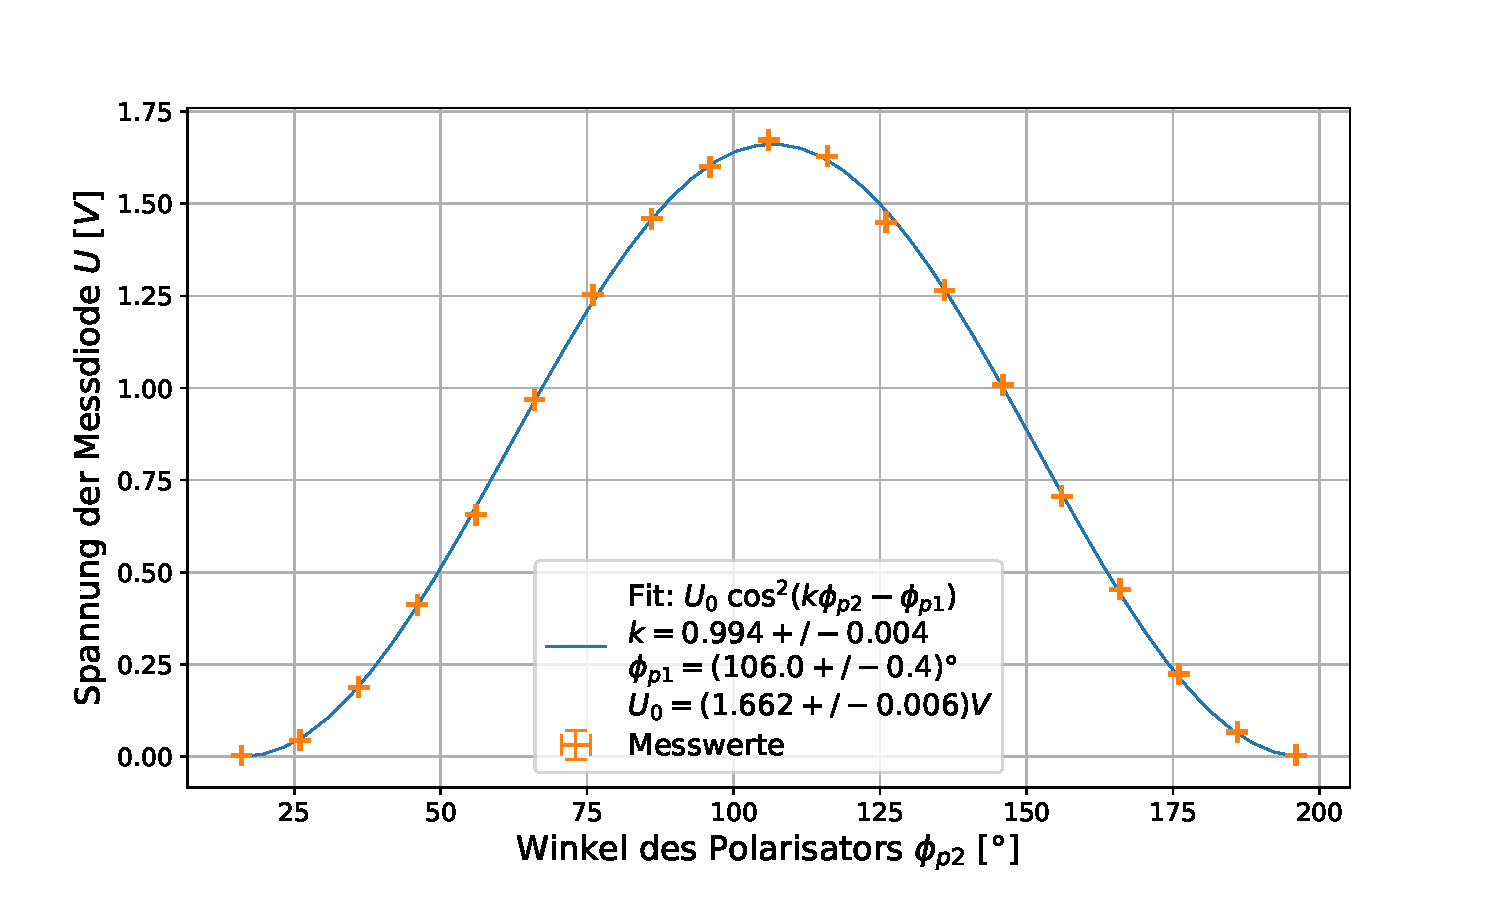
\includegraphics[width=\textwidth]{data/laserPolarisation.pdf}
				\caption{Messpunkte für die Polarisation und $\cos^2$-Fit zur Überprüfung des Gesetzes von Malus.}
				\label{fig:PolarisationFit}	
			\end{figure}
			Über die Messpunkte in Abb. \ref{fig:PolarisationFit} wurde zusätzlich ein $\cos^2$-Fit gelegt, um die Form des Gesetzes von Malus zu überprüfen.
			Der Fit verläuft dabei durch jeden Messpunkt bzw. einer Unsicherheit dieser Punkte.
			Für $U_0$ steht an der Stelle in dem Fit $A = \SI{1,662+-0,006}{\volt}$, für den Ausgangswinkel wie zuvor $\phi_0 = \SI{106+-0,4}{\degree}$.
			Hinzu kommt der Korrekturfaktor $k=0,994+-0,004$ vor der Drehung um den Winkel $\phi$, da $A$ ansonsten von $U_0$ abweichen würde.
		
		\subsubsection*{Diskussion}
			
			Nun zu der Überprüfung der Hypothese, dass die Ergebnisse dieses Teilversuches mit dem Gesetz von Malus übereinstimmen.
			Die Größe $k$ wird hierfür als 1 angenommen, da nahezu keine Abweichung davon vorliegt und nur dem Fit dient.
			Da die Messpunkte alle auf dem $\cos^2$-Fit liegen und die Intensität $I$ proportional zu der gemessenen Spannung $U$ ist, lässt sich die Hypothese bestätigen.
			Auch ohne Einstrahlung des Laserlichts von außen eine geringfügige Spannung von \SI{3+-0,21}{\milli\volt} durch das Licht in dem Raum aufgenommen wurde, diese hatte jedoch keinen nennenswerten Einfluss auf das Ergebnis.
